\documentclass[border=4pt,12pt]{standalone}
% House style for redrawn exam diagrams (diagram-v4: 0.4pt lines, filled -latex arrows, fine dashes; stipple and hatching drawn as real dots/lines (no PDF/SVG patterns, so they render in every browser and at any scale); transparent background). Every figure \input's this.
\usepackage{amsmath,amssymb}
\usepackage{txfonts}
\usepackage{pdfrender,xcolor}
% \halo{text}: label on shading. The shading stops just around each letter's outline (a thin knock-out that follows the
% glyphs, like the papers' typesetting), never a box. Owner: "I don't want a box around the text".
\newcommand{\halo}[1]{\leavevmode\rlap{\pdfrender{TextRenderingMode=2,LineWidth=2.2pt,LineJoinStyle=1,StrokeColor=white,FillColor=white}#1}#1}
\usepackage{tikz,pgfplots}
\pgfplotsset{compat=1.18}
\usetikzlibrary{arrows.meta,calc,angles,quotes,patterns,patterns.meta,intersections,positioning,decorations.markings,shapes.geometric}
% Stipple and hatching are drawn as actual dots / lines clipped to the region (path picture), NOT as pattern fills:
% SVG <pattern> fills vanish or blur when browsers scale the image, so the owner could not see the shading.
% Each dot is a 0.72pt square (keeps SVGs small; reads as a dot at print size). Dots sit on one global staggered grid, so neighbouring regions line up.
\makeatletter
\newdimen\ex@x \newdimen\ex@y \newdimen\ex@xa \newdimen\ex@ya \newdimen\ex@xb \newdimen\ex@yb \newcount\ex@row
\def\exam@stipplecolor{black!75}\def\exam@dotr{0.42pt}\def\exam@dotgap{2.5}
\def\ex@rowdots{\ifdim\ex@x<\ex@xb \pgfpathrectangle{\pgfqpoint{\dimexpr\ex@x-0.36pt\relax}{\dimexpr\ex@y-0.36pt\relax}}{\pgfqpoint{0.72pt}{0.72pt}}\advance\ex@x by \exam@dotgap pt\relax\expandafter\ex@rowdots\fi}
\def\exam@stipple{%
  \pgftransformreset% dots are sized in real points even inside scaled pictures
  \pgfpointanchor{path picture bounding box}{south west}\ex@xa=\pgf@x \ex@ya=\pgf@y
  \pgfpointanchor{path picture bounding box}{north east}\ex@xb=\pgf@x \ex@yb=\pgf@y
  \pgfsetfillcolor{\exam@stipplecolor}\pgfmathsetmacro\ex@h{\exam@dotgap/2}%
  \pgfmathtruncatemacro\ex@r{floor(\ex@ya/\ex@h)-1}\ex@row=\ex@r\relax
  \ex@y=\ex@r\dimexpr\ex@h pt\relax
  \loop\ifdim\ex@y<\ex@yb
    \pgfmathtruncatemacro\ex@c{floor(\ex@xa/\exam@dotgap)-1}\ex@x=\ex@c\dimexpr\exam@dotgap pt\relax
    \ifodd\ex@row \advance\ex@x by \ex@h pt\fi
    \ex@rowdots
    \advance\ex@y by \ex@h pt \advance\ex@row by 1
    \ifnum\numexpr\ex@row-(\ex@row/4)*4\relax=0 \pgfusepath{fill}\fi% flush every 4 rows: bounded TeX memory, few clip copies in the SVG
  \repeat\pgfusepath{fill}}
\newdimen\ex@d
\def\exam@hatch#1{% #1 = 1 for /, -1 for \ ; lines 45 degrees, 3pt apart
  \pgftransformreset
  \pgfpointanchor{path picture bounding box}{south west}\ex@xa=\pgf@x \ex@ya=\pgf@y
  \pgfpointanchor{path picture bounding box}{north east}\ex@xb=\pgf@x \ex@yb=\pgf@y
  \ex@d=\dimexpr\ex@yb-\ex@ya\relax \ex@x=\dimexpr\ex@xa-\ex@d\relax
  \loop\ifdim\ex@x<\ex@xb
    \ifnum#1>0 \pgfpathmoveto{\pgfqpoint{\ex@x}{\ex@ya}}\pgfpathlineto{\pgfqpoint{\dimexpr\ex@x+\ex@d\relax}{\ex@yb}}%
    \else \pgfpathmoveto{\pgfqpoint{\ex@x}{\ex@yb}}\pgfpathlineto{\pgfqpoint{\dimexpr\ex@x+\ex@d\relax}{\ex@ya}}\fi
    \advance\ex@x by 4.24pt
  \repeat
  \pgfsetlinewidth{0.4pt}\pgfsetstrokecolor{black}\pgfusepath{stroke}}
\def\examstipple{\exam@stipple}\def\examhatch{\exam@hatch}\def\examsetstipplecolor#1{\def\exam@stipplecolor{#1}}\def\examsetdotgap#1{\def\exam@dotgap{#1}}
\makeatother
% (legacy pattern kept for old files)
% staggered stipple like the NESA papers' dotted shading
\pgfdeclarepatternformonly{exam stipple}{\pgfpointorigin}{\pgfqpoint{2.2pt}{2.2pt}}{\pgfqpoint{2.2pt}{2.2pt}}{%
  \pgfpathcircle{\pgfqpoint{0.55pt}{0.55pt}}{0.42pt}\pgfpathcircle{\pgfqpoint{1.65pt}{1.65pt}}{0.42pt}\pgfusepath{fill}}
\tikzset{
  every picture/.style={line width=0.6pt, >={Latex[length=2mm,width=1.3mm]}},
  curve/.style={line width=0.6pt},
  open arrow/.style={-{Latex[length=2mm,width=1.3mm]}},  % owner: filled -latex heads everywhere, no open chevrons
  aux/.style={dash pattern=on 2pt off 1.5pt, line width=0.6pt},
  shade/.code={\def\exA{#1}\def\exB{none}\ifx\exA\exB\else\pgfkeysalso{fill=black!18}\fi},
  shade/.default=on,
  shade dots/.style={fill=none, path picture={\examstipple}},
  stipple color/.code={\examsetstipplecolor{#1}},
  stipple gap/.code={\examsetdotgap{#1}},
  shade dense dots/.style={fill=none, stipple gap=1.6, path picture={\examstipple}},
  shade hatch/.style={fill=none, path picture={\examhatch{1}}},
  shade hatch reverse/.style={fill=none, path picture={\examhatch{-1}}},
  shade solid/.style={fill=black},
  pt/.style={circle, fill, inner sep=1.1pt},
  open pt/.style={circle, draw, fill=white, inner sep=1.1pt},
}
\pgfplotsset{
  exam axes/.style={axis lines=middle, axis line style={->}, xlabel={$x$}, ylabel={$y$},
    xlabel style={anchor=west}, ylabel style={anchor=south}, tick label style={font=\small},
    every axis plot/.append style={line width=0.6pt, black}, samples=200, clip=false,
    enlargelimits=false, axis on top},
}

\begin{document}
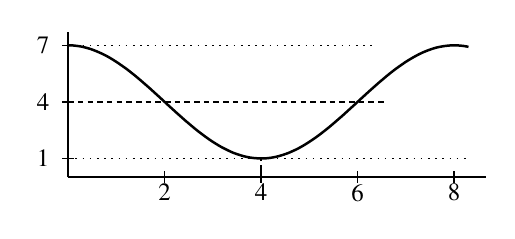
\begin{tikzpicture}[x=0.0127cm,y=-0.0127cm]
\draw (54.0,232.0) -- (472.0,232.0);
\draw (54.0,232.0) -- (54.0,86.8);
\draw (150.5,232.0) -- ++(0,-6) node[below=1pt,font=\small] {$2$}; \draw (150.5,232.0) -- ++(0,6);
\draw (247.0,232.0) -- ++(0,-6) node[below=1pt,font=\small] {$4$}; \draw (247.0,232.0) -- ++(0,6);
\draw (343.5,232.0) -- ++(0,-6) node[below=1pt,font=\small] {$6$}; \draw (343.5,232.0) -- ++(0,6);
\draw (440.0,232.0) -- ++(0,-6) node[below=1pt,font=\small] {$8$}; \draw (440.0,232.0) -- ++(0,6);
\draw (54.0,213.1) -- ++(-6,0) node[left=1pt,font=\small] {$1$}; \draw (54.0,213.1) -- ++(6,0);
\draw (54.0,156.6) -- ++(-6,0) node[left=1pt,font=\small] {$4$}; \draw (54.0,156.6) -- ++(6,0);
\draw (54.0,100.0) -- ++(-6,0) node[left=1pt,font=\small] {$7$}; \draw (54.0,100.0) -- ++(6,0);
\draw[dotted] (54.0,100.0) -- (358.0,100.0); \draw[dotted] (54.0,213.1) -- (454.5,213.1);
\draw[aux] (54.0,156.6) -- (372.4,156.6);
\draw[aux] (247.0,225.4) -- (247.0,213.1);
\draw[line width=0.9pt] plot[smooth] coordinates {(54.0,100.0) (58.5,100.1) (63.0,100.6) (67.5,101.3) (72.0,102.4) (76.5,103.7) (81.0,105.4) (85.5,107.3) (90.0,109.4) (94.5,111.8) (99.0,114.5) (103.5,117.4) (108.0,120.5) (112.5,123.7) (117.0,127.2) (121.5,130.8) (126.0,134.6) (130.5,138.5) (135.0,142.4) (139.5,146.5) (144.0,150.6) (148.5,154.7) (153.0,158.9) (157.5,163.0) (162.0,167.1) (166.5,171.1) (171.0,175.1) (175.5,178.9) (180.0,182.7) (184.5,186.3) (189.0,189.7) (193.5,193.0) (198.0,196.1) (202.5,198.9) (207.0,201.6) (211.5,203.9) (216.0,206.1) (220.5,208.0) (225.0,209.5) (229.5,210.9) (234.0,211.9) (238.5,212.6) (243.0,213.0) (247.5,213.1) (252.0,213.0) (256.5,212.5) (261.0,211.7) (265.5,210.6) (270.0,209.2) (274.5,207.6) (279.0,205.6) (283.5,203.5) (288.0,201.0) (292.5,198.3) (297.0,195.4) (301.5,192.3) (306.0,189.0) (310.5,185.5) (315.0,181.9) (319.5,178.1) (324.0,174.2) (328.5,170.3) (333.0,166.2) (337.5,162.1) (342.0,158.0) (346.5,153.8) (351.0,149.7) (355.5,145.6) (360.0,141.6) (364.5,137.6) (369.0,133.8) (373.5,130.0) (378.0,126.4) (382.5,123.0) (387.0,119.8) (391.5,116.7) (396.0,113.9) (400.5,111.3) (405.0,108.9) (409.5,106.8) (414.0,105.0) (418.5,103.4) (423.0,102.1) (427.5,101.2) (432.0,100.5) (436.5,100.1) (441.0,100.0) (445.5,100.2) (450.0,100.7) (454.5,101.5)};
\end{tikzpicture}
\end{document}
